\section{Refactoring (8P)}
\subsection{Code Smells (2P)}
\task{jeweils 1 Code-Beispiel zu 2 unterschiedlichen Code Smells (die benannt werden müssen) aus der Vorlesung; jeweils Code-Beispiel und einen möglichen Lösungsweg bzw. den genommen Lösungsweg beschreiben (inkl. (Pseudo-)Code)}
\subsubsection*{Code Smell 1: Duplicated Code \textit{main/Commit bc6ad15}}
\todo{Sollte eigentlich OK sein, aber ich bin kein Fän davon, dass wir hier das gleiche Beispiel von DRY nutzen}
\subsubsection*{Vorher}
\lstinputlisting[language=Java,style=codeStyle]{kapitel7_refactoring/codesmell1.java}
\subsubsection*{Lösung}
Der Code Smell wurde gelöst, indem die Methode \textit{convertCurrency(String currencyCode, String currencyName)} eingeführt wurde. Diese wird in den einzelnen Methoden für die jeweilige Währung aufgerufen.
\lstinputlisting[language=Java,style=codeStyle]{kapitel7_refactoring/codesmell2.java}


\subsubsection*{Code Smell 2: Switch-Statement \textit{main/Commit c46c962}}
\subsubsection*{Vorher}
\lstinputlisting[language=Java,style=codeStyle]{kapitel7_refactoring/codesmell3.java}

\subsubsection*{Lösung}
Dadurch das bei weiteren Commands das Switch-Statement komplexer geworden wäre, wurde es durch eine Hash-Map ersetzt für mehr flexibilität. Dazu wurde nun auch der Code für die Commands in eigene Klassen ausgelagert. Das hat generll auch zu einer verbesserten lesbarkeit gewirkt.
\lstinputlisting[language=Java,style=codeStyle]{kapitel7_refactoring/codesmell4.java}
\newpage
\subsection{2 Refactorings (6P)}
\task{2 unterschiedliche Refactorings aus der Vorlesung jeweils benennen, anwenden, begründen, sowie UML vorher/nachher liefern; jeweils auf die Commits verweisen – die Refactorings dürfen sich nicht mit den Beispielen der Code überschneiden}

\subsubsection*{Refactoring 1: Replace Error Code with Exceptions \textit{main/Commit 2cc1fce}} 
Alle Methoden von UserService werfen eine DatabaseException die nicht abgefangen wurde. Daher wurden try-catch-Block um die jeweiligen Methoden hinzugefügt.


\begin{figure}[h!]
    \centering
    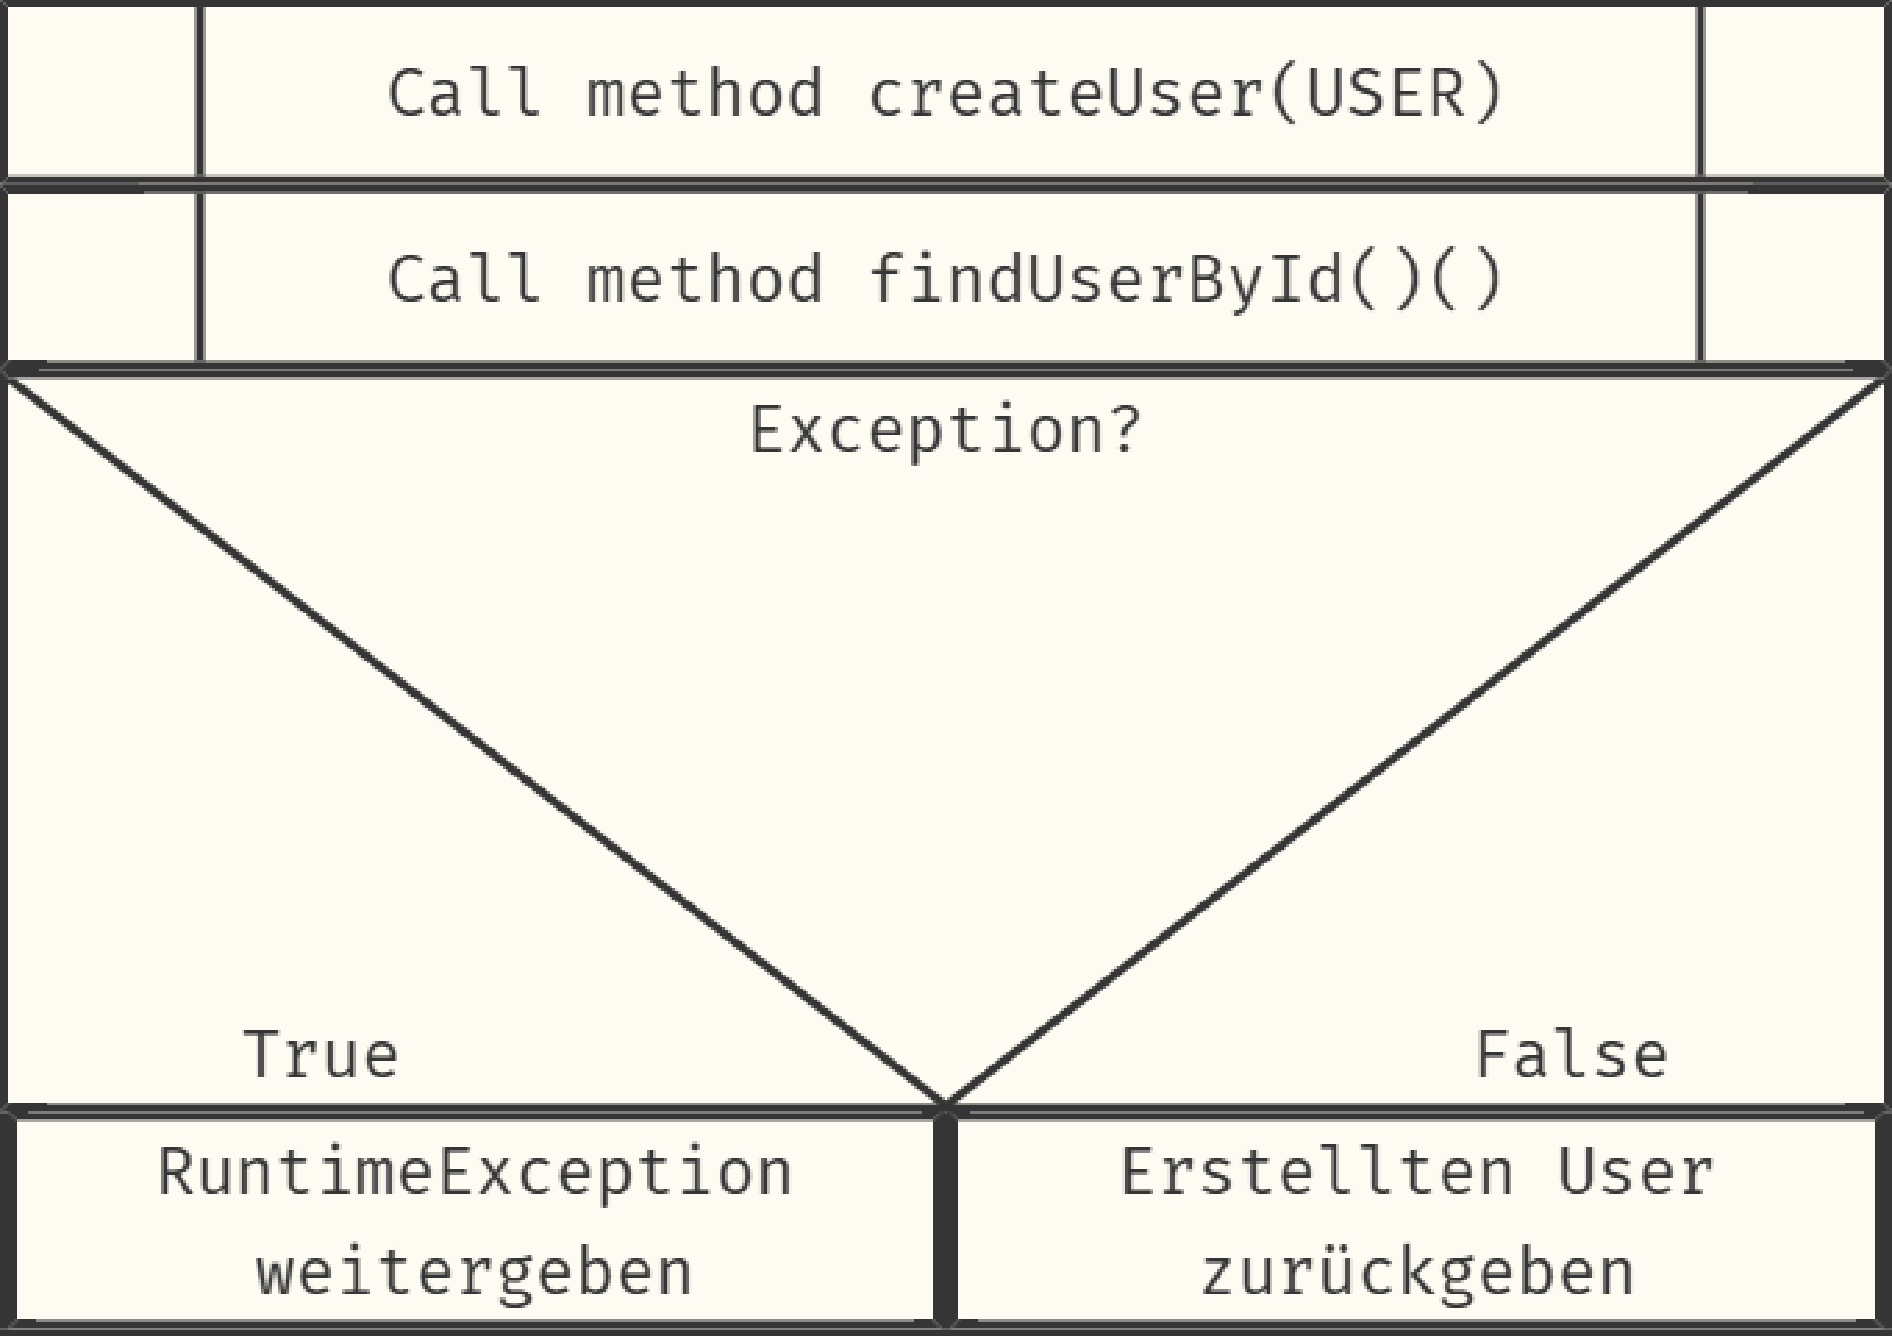
\includegraphics[width=0.75\linewidth]{kapitel7_refactoring/ref_before.pdf}
    \caption{SignUp\#register vorher}
\end{figure}


\begin{figure}[h!]
    \centering
    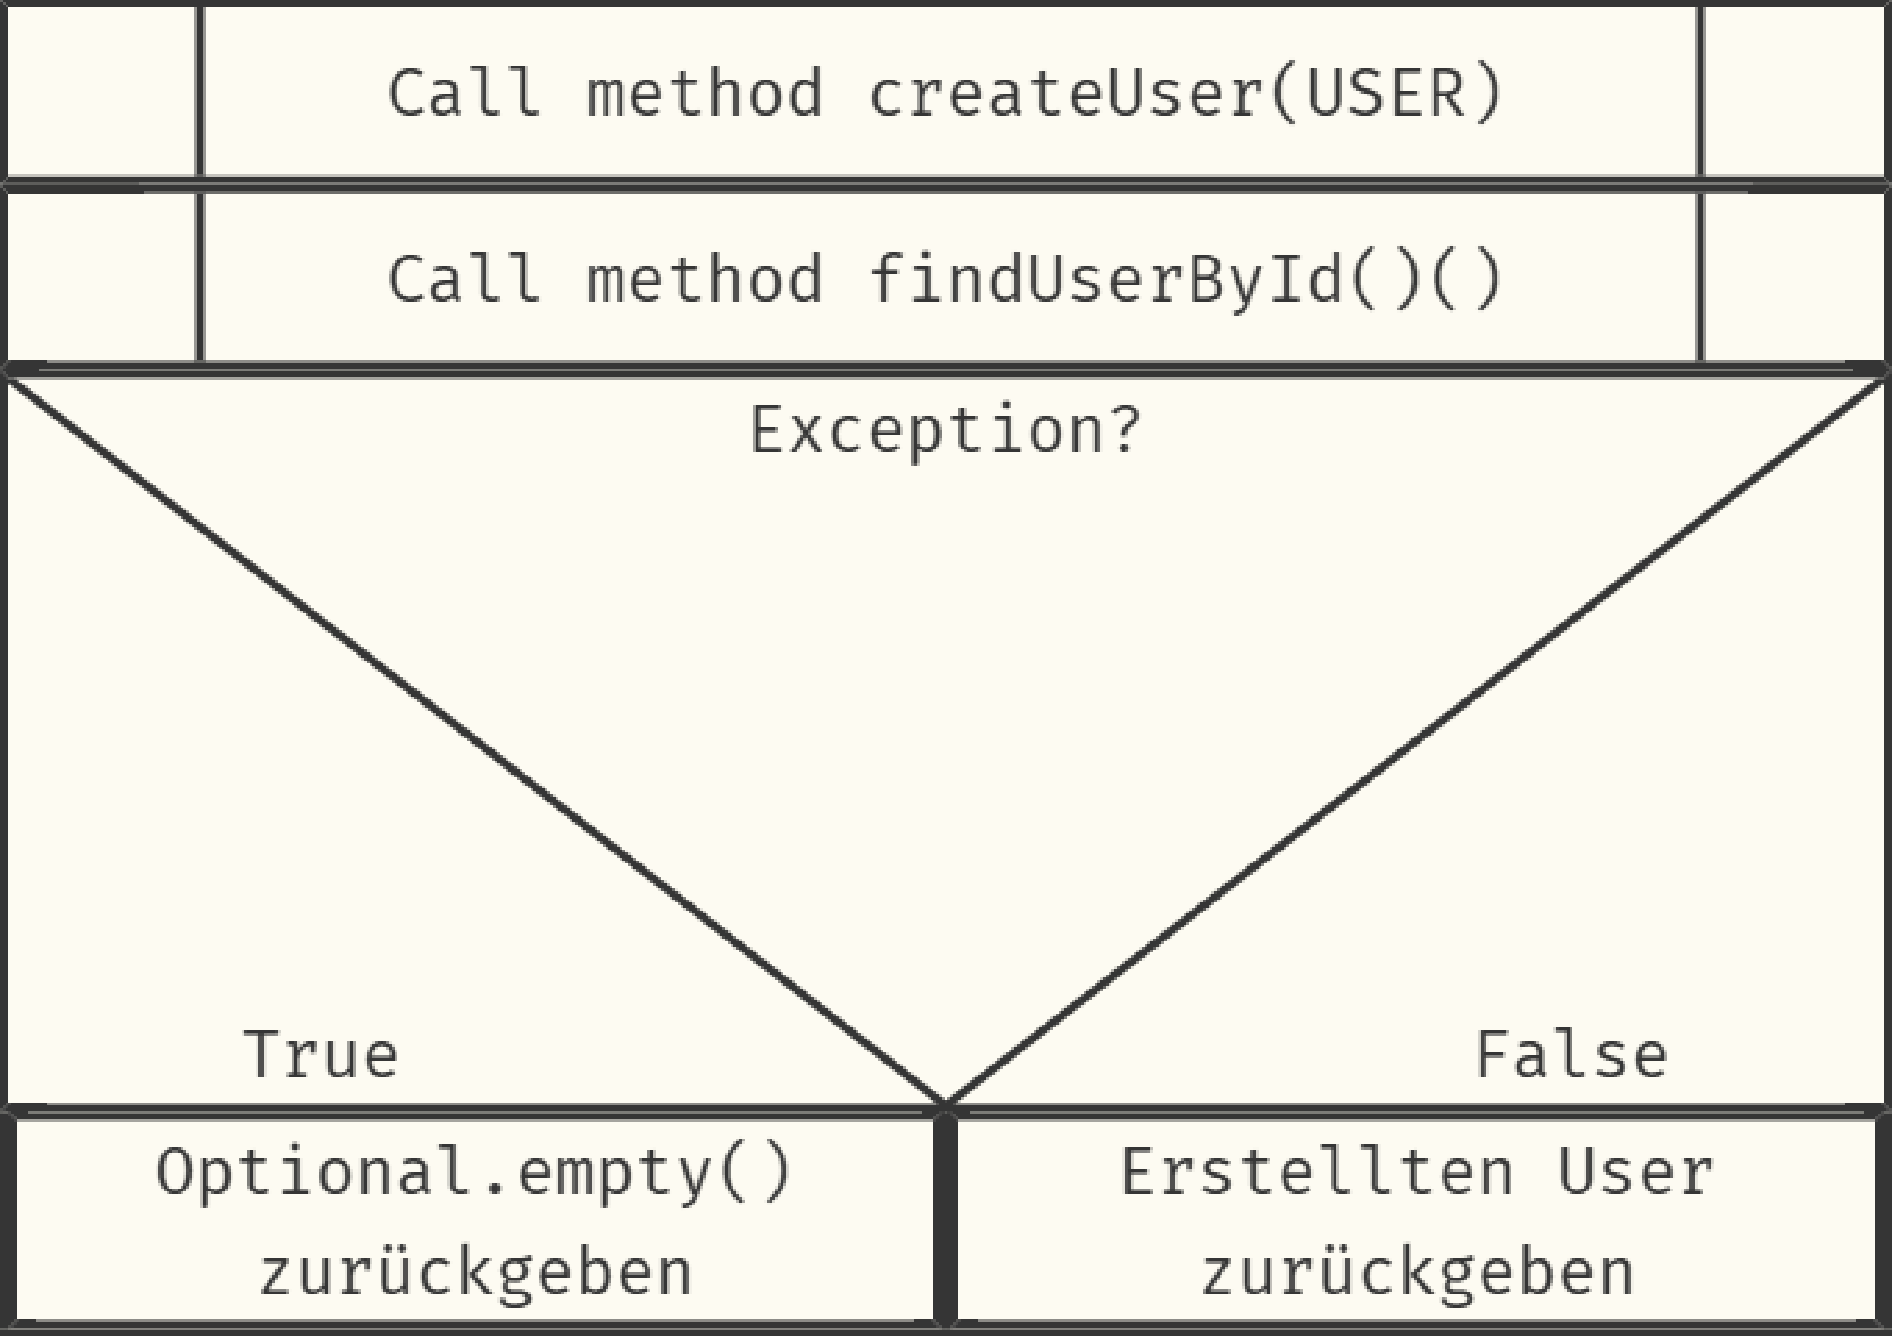
\includegraphics[width=0.75\linewidth]{kapitel7_refactoring/ref_after.pdf}
    \caption{SignUp\#register nachher}
\end{figure}
 \newpage
\subsubsection*{Refactoring 2: Rename Methods \textit{main/Commit d3be454}}
Die Methode login() in der Klasse SignUp wurde zu waitUntilLoggedIn() umbenannt da in der Methode erwartet wird bis der Benutzter eingeloggt ist und daraufhin dann entscheidet.
\newline\newline
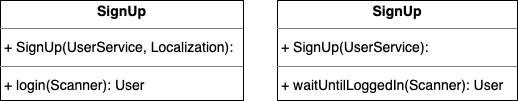
\includegraphics[width=\linewidth]{kapitel7_refactoring/Refactor2.png}
 